\documentclass{article}
\usepackage[utf8]{inputenc}
\usepackage[english]{babel}
\usepackage[]{amsthm} 
\usepackage[]{amssymb} 
\usepackage{amsmath}
\usepackage{graphicx}
\graphicspath{ {./prob1_images/} }
\usepackage{hyperref}
\usepackage{mathtools}
\usepackage[thinc]{esdiff}
\usepackage[dvipsnames]{xcolor}
\usepackage{float}
\newtheorem*{theorem}{Theorem}

\title{ADSP: HW2}
\author{Lo Chun, Chou \\ R13922136}
\date\today


\begin{document}
\setlength{\parindent}{0pt}
\maketitle 

\section*{(1)}

The resulting plot using $k = 8$ is shown in the below figure:

\begin{figure}[H]
    \centering
    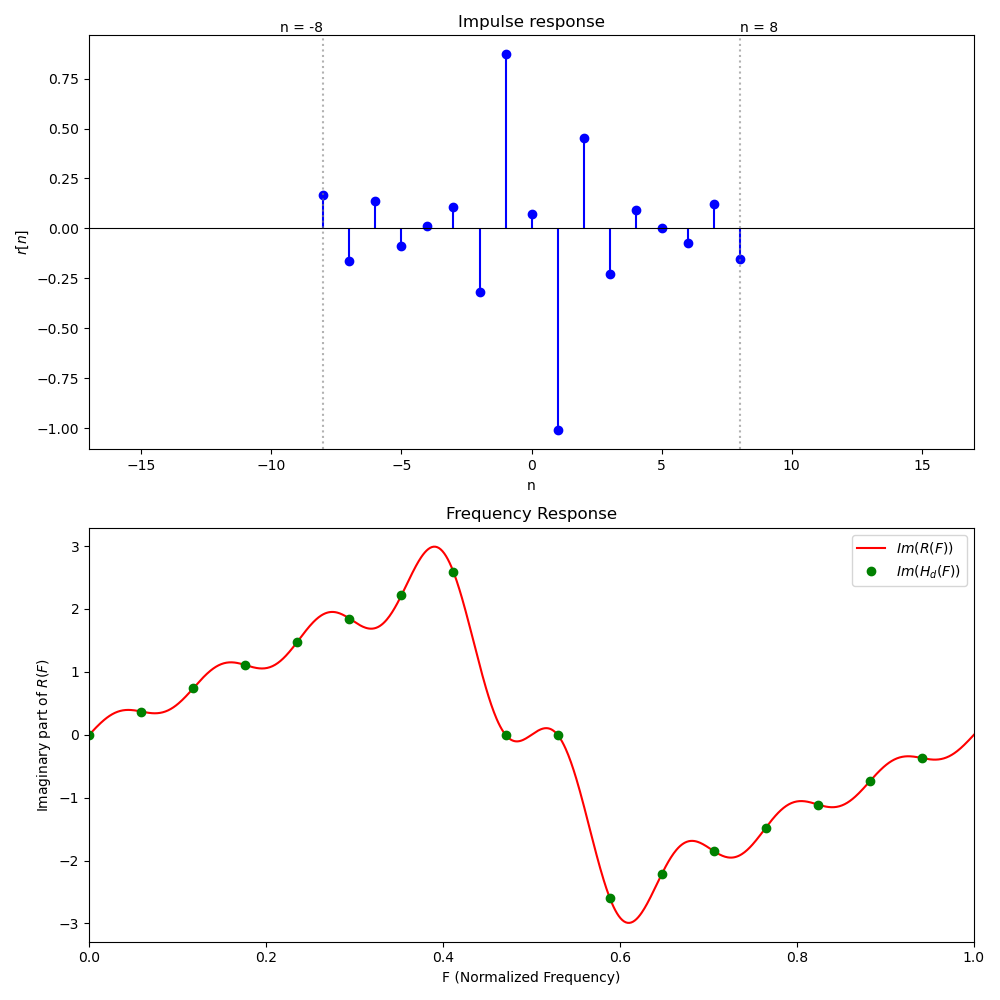
\includegraphics[width=0.9\textwidth]{prob1_images/required_plot.png}
    \caption{The resulting plot using $k = 8$}
\end{figure}

\section*{(2)}
\subsection*{(a)}

\begin{enumerate}
    \item All the poles and the zeros are within the unit circle, 
    so this makes both the forward and inverse transform stable.  
    \item It makes the impulse response concentrated around $0$.
\end{enumerate}

\subsection*{(b)} 

Hilbert transform takes more sample points into consideration, rather than relying on just two.
\bigskip

Therefore, compared to the difference-based approach, which only considers two points, Hilbert transform is less sensitive to noise.
This means that if there is noise, the difference method may fail to clearly distinguish the signal’s edges,
whereas the Hilbert transform can still effectively find them.

\subsection*{(c)}

Weiner's filter design the filter based on statistics, so compared to the pass-stop band filter,
it can better decide the passband and stopband.
\bigskip

For example, when we use pass-stop band filter to preserve only people's voice,
we set $f > 3000 Hz$ as the stopband, but in fact, 
for some frequency over $3000 Hz$, there could still be human voice, 
and for some frequency under $3000 Hz$, there could be sounds that are not human, for example, car honk sound.
\bigskip

To conclude, Weiner's filter uses experiments to replace using our knowledge about what our system should be. 
(We don't need to assume the value $3000 Hz$ to be the cutoff frequency.)

\subsection*{(d)}

\begin{enumerate}
    \item We do not need to know the values of $\alpha_i$ when using cepstrum.
    \item We do not need to know the values of $\tau_j$ when using cepstrum.
\end{enumerate}

Also, the values for $\alpha_i$ and $\tau_j$ would change when the environment changes, 
so the equalizer approach is not suitable for wireless communication, while using cepstrum can avoid these problems.

\section*{(3)}

It is improper to use this approach because the complexity of DFT is $\theta(N log_2 N)$,
and the complexity of other FIR methods is $\theta(N)$.  
\bigskip 

Therefore, the computation cost is too high to use this method, for example, 
because we need to satisfy the Nyquist criterion, $fs > 2B$, so for an audio signal with $B = 21000 Hz$, 
we need to do fourier transform and inverse fourier transform for over fourty thousand samples for 10 seconds.

\section*{(4)}

\subsection*{(a)}

We can use the weight function to control accuracy at different frequency bands in FIR filter design.  
We set $W(f) = 1$ for the more important part and $0 < W(f) < 1$ for the less important part.  
\bigskip

For example, if the passband is treated to be more important, 
then $W(f) = 1$ in the passband, and $0 < W(f) < 1$ in the stopband.


\subsection*{(b)}

\subsubsection*{(i)}

Yes, the weight function can be applied in the FIR filter design by the MSE method.  

\subsubsection*{(ii)}

No, the weight function cannot be applied in the FIR filter design by the frequency sampling method.  

\section*{(5)}

From ppt p.149 we knew that any odd function that has its energy decrease as $|n|$ increases can be seen as an edge detection filter.
Therefore, we should only choose from $(ii), (iv)$.

\subsection*{(a)}

$(ii)$ changes sharply at the symmetric center, and stays at $0$ at the two sides,
this means that it only considers the small part around the center,
which is suitable for extracting small scaled features.

\subsection*{(b)}

$(iv)$ gradually decreases as $|n|$ increases,
this means that it takes more sample points into consideration,
so it is suitable for extracting large-scaled features.

\section*{(6)}

\subsection*{(a)}

First we factor the denominator by finding its roots:

\begin{align*}
    z = \{\frac{0.7 \pm \sqrt{0.49 - 0.4}}{2}\} = \frac{0.7 \pm 0.3}{2} = \{0.5, 0.2\}
\end{align*}

And the numerator, we knew that the roots could be $\{\pm \frac{1}{2}, \pm 1, \pm 2\}$:

\begin{align*}
    z = \frac{1}{2} &: \quad 2z^3 - 2z^2 -3z - 2 = \frac{2}{8} - \frac{2}{4} - \frac{3}{2} - 2 = -\frac{15}{4} \\
    z = -\frac{1}{2} &: \quad 2z^3 - 2z^2 -3z - 2 = -\frac{2}{8} - \frac{2}{4} + \frac{3}{2} - 2 = -\frac{10}{8} \\
    z = 1 &: \quad 2z^3 - 2z^2 -3z - 2 = 2 - 2 - 3 - 2 = -5 \\
    z = -1 &: \quad 2z^3 - 2z^2 -3z - 2 = - 2 - 2 + 3 - 2 = -3 \\
    \textcolor{Green}{z = 2} &: \quad 2z^3 - 2z^2 -3z - 2 = 16 - 8 - 6 - 2 = 0 \\
    z = -2 &: \quad 2z^3 - 2z^2 -3z - 2 = -16 - 8 + 6 - 2 = -20
\end{align*}

Then we have:

\begin{align*}
    z^3 - 2z^2 -3z - 2 \div (z - 2) = 2z^2 + 2z + 1
\end{align*}

The roots of $2z^2 + 2z + 1$ are $\{\frac{-1 \pm j}{2}\}$

Therefore, $H(z)$ is:

\begin{align*}
    H(z) = \frac{(z - 2)(z - \frac{-1 + j}{2})(z - \frac{-1 - j}{2})}{(z - 0.5)(z - 0.2)} 
\end{align*}

The poles and zeros are:

\begin{align*}
    \text{poles} &= \{0.5, 0.2\} \\
    \text{zeros} &= \{\textcolor{red}{2}, \frac{-1 + j}{2}, \frac{-1 - j}{2}\}
\end{align*}

Since only $|2| > 1$ is not within the unit circle, 
we can convert $H(z)$ into a minimum phase filter $H_1(z)$ as follows:

\begin{align*}
    H_1(z) 
    &= \frac{(z - 2)(z - \frac{-1 + j}{2})(z - \frac{-1 - j}{2})}{(z - 0.5)(z - 0.2)} \textcolor{orange}{\times 2 \frac{(z - 0.5)}{(z - 2)}} \\
    &= \textcolor{orange}{2} \frac{\textcolor{orange}{(z - 0.5)}(z - \frac{-1 + j}{2})(z - \frac{-1 - j}{2})}{(z - 0.5)(z - 0.2)(z - 2)}
\end{align*}

\subsection*{(b)}

From the previous subsection, we have:

\begin{align*}
    H_1(z) = 2 \frac{(z - 0.5)(z - \frac{-1 + j}{2})(z - \frac{-1 - j}{2})}{(z - 0.5)(z - 0.2)(z - 2)}
\end{align*}

This is equivalent to:

\begin{align*}
    H(z) = z^{3 - 2} \times 2 \times \frac{(z - 0.5)(1 - \frac{-1 + j}{2}z^{-1})(1 - \frac{-1 - j}{2}z^{-1})}{(1 - 0.5z^{-1})(1 - 0.2z^{-1})} 
\end{align*}

Using the notations of ppt p.186, we have:

\begin{itemize}
    \item zeros inside the unit circle: $a_1 = \frac{-1 + j}{2}, \ a_2 = \frac{-1 - j}{2}$
    \item zeros outside the unit circle: $b_1^{-1} = 2 \ (b_1 = 0.5)$
    \item poles inside the unit circle: $c_1 = 0.5, \ c_2 = 0.2$
    \item $A = 2$
\end{itemize}

By directly using the formula of ppt p.188, we would get the cepstrum:

\begin{equation*}
\hat{x}[n] = 
    \begin{cases}
    log(A) = log(2) \qquad &,n = 0\\
    - \frac{a_1^n}{n} - \frac{a_2^n}{n} + \frac{c_1^n}{n} + \frac{c_2^n}{n} = - \frac{(\frac{-1 + j}{2})^n}{n} - \frac{(\frac{-1 - j}{2})^n}{n} + \frac{(0.5)^n}{n} + \frac{(0.2)^n}{n} \qquad &,n > 0\\
    \frac{b_1^n}{n} =  \frac{(0.5)^n}{n} \qquad &,n < 0\\
    \end{cases}
\end{equation*}

\section*{(7)}

Since we're given:

\begin{equation*}
\hat{x}[n] = 
    \begin{cases}
    0.8 \qquad &,n = 2 \\
    0 &, \text{otherwise}
\end{cases}
\end{equation*}

We can write:

\begin{align*}
    \hat{x}[n] = 0.8 \delta[n - 2]
\end{align*}

Then take the z transform, and using the property that $\delta[n - m] \Rightarrow z^{-m}$, we have:

\begin{align*}
    \hat{X}(z) = Z[\hat{x}[n]] = \sum_{n=-\infty}^{\infty} \hat{x}[n] z^{-n} = 0.8 z^{-2}
\end{align*}

Since $\log X(z) = \hat{X}(z)$:

\begin{align*}
    \log X(z) = 0.8 z^{-2}
\end{align*}

Taking exponential on both sides:

\begin{align*}
    X(z) = e^{0.8 z^{-2}}
\end{align*}

Using the formula $e^x = \sum_{n=0}^{\infty} \frac{x^n}{n!}$:

\begin{align*}
    X(z) = \sum_{n=0}^{\infty} \frac{(0.8 z^{-2})^n}{n!} = \sum_{n=0}^{\infty} \frac{0.8^n}{n!} z^{-2n}
\end{align*}

The z-transform of $x[n]$ is $X(z)$, and change the variable for the later from $n$ to $k$ to increase readability:

\begin{align*}
    x[n] = \sum_{n=0}^{\infty}x[n] z^{-n} = \sum_{k=0}^{\infty} \frac{0.8^k}{k!} z^{-2k}
\end{align*}

Therefore we have:

\begin{equation*}
x[n] = 
    \begin{cases}
    \frac{0.8^k}{k!} \qquad &,n = 2k, k = 0, 1, 2, \cdots \\
    0 &, \text{otherwise}
    \end{cases}
\end{equation*}




\section*{Extra (ended with (1, 6))}

The discrete Hilbert transform has another application, which is analytic function.
\bigskip

By using the analytic function to generate single-sided band signal, since the positive part is the same as the negative part
(for real $x[n], \ X(F) = X^*(-F)$),
we can neglect the negative part (because it can be reconstructed by the positive part) and only record the positive part.
\bigskip

Also, when sending the signal, we only need to send the positive part.


\end{document}